% ++++++++++++ Controller PSoC Master klassen ++++++++++++++
\subsubsection{Domain-klasse: Data}
q
\begin{figure}[h]
\centering
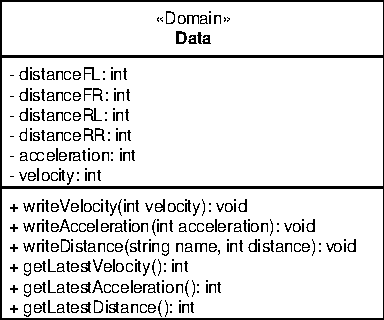
\includegraphics[]{../fig/diagrammer/bil/cd_data.pdf}
\caption{Klassebeskrivelse for domain-klassen Data}
\label{fig:cd_data}
\end{figure}
%TODO opdater pdf

\textbf{Attributter}

\begin{table}[h]
\begin{tabularx}{\textwidth}{| Z | Z | L{10cm} |} \hline
Navn & Type & Beskrivelse \\\hline

\texttt{distanceFL} & \texttt{int} &Variabel der indeholder afstanden til en evt. forhindring ved forreste venstre hjørne af bilen i cm.\\\hline

\texttt{distanceFR} & \texttt{int} &Variabel der indeholder afstanden til en evt. forhindring ved forreste højre hjørne af bilen i cm.\\\hline

\texttt{distanceRL} & \texttt{int} &Variabel der indeholder afstanden til en evt. forhindring ved bageste venstre hjørne af bilen i cm.\\\hline

\texttt{distanceRR} & \texttt{int} &Variabel der indeholder afstanden til en evt. forhindring ved bageste højre hjørne af bilen i cm.\\\hline

\texttt{acceleration} & \texttt{int} &Variabel der indeholder bilens aktuelle acceleration i $G / 10$.\\\hline

\texttt{velocity} & \texttt{int} &Variabel der indeholder bilens aktuelle hastighed i $(km/t)/ 10$.\\\hline

\texttt{Input} & \texttt{UserInput} &En struct der der indeholder userinput til systemet. Denne struct er specificeret i utilities.hpp.\\\hline

\texttt{myLog} & \texttt{Log*} &En pointer til systemets log.\\\hline

\texttt{sensorDataMut} & \texttt{std::mutex} &En mutex der anvendes som lås til de variable der skal indeholde data fra alle bilens sensorer.\\\hline

\texttt{userDataMut} & \texttt{std::mutex} &En mutex der anvendes som lås til de variable der skal indeholde data om brugerens input.\\\hline

\end{tabularx}
\caption{Attributter for klassen Data}
\label{table:attr_data}
\end{table}
%TODO ret enheder i ovenstående

\textbf{Metoder}
%------------------------------------- writeVelocity -------------------------------------
\begin{table}[h]
\begin{tabularx}{\textwidth}{| L{2.5 cm} | Z |} \hline
Prototype & \texttt{bool writeVelocity(int velocity)} \\\hline
Parametre & \texttt{velocity} \newline Den hastighed der skal indlæses. \\\hline
Returværdi &  \texttt{bool} \newline Returnerer \texttt{true} hvis skrivningen er gået godt og \texttt{false} hvis skrivningen gik galt. \\\hline
Beskrivelse & Metoden indlæser den nyeste værdi af hastigheden i datastrukturen. \\\hline
\end{tabularx}
\caption{Metodebeskrivelse for \texttt{writeVelocity}}
\label{table:met_writeVelocity}
\end{table}

%------------------------------------- writeAcceleration -------------------------------------
\begin{table}[h]
\begin{tabularx}{\textwidth}{| L{2.5 cm} | Z |} \hline
Prototype & \texttt{bool writeAcceleration(int acceleration)} \\\hline
Parametre & \texttt{acceleration} \newline Den acceleration der skal indlæses. \\\hline
Returværdi &  \texttt{bool} \newline Returnerer \texttt{true} hvis skrivningen er gået godt og \texttt{false} hvis skrivningen gik galt. \\\hline
Beskrivelse & Metoden indlæser den nyeste værdi af accelerationen i datastrukturen. \\\hline
\end{tabularx}
\caption{Metodebeskrivelse for \texttt{writeAcceleration}}
\label{table:met_writeAcceleration}
\end{table}

%------------------------------------- writeDistance -------------------------------------
\begin{table}[h]
\begin{tabularx}{\textwidth}{| L{2.5 cm} | Z |} \hline
Prototype & \texttt{bool  writeDistance(string name, int distance)} \\\hline
Parametre & \texttt{name} \newline Navnet på den sensor som der skal indlæses data fra. Kan være FL, FR, RL eller RR. \newline \newline
			\texttt{distance} \newline
			Afstanden der fra den pågældende sensor der skal indlæses i datastrukturen.\\\hline
Returværdi &  \texttt{bool} \newline Returnerer \texttt{true} hvis skrivningen er gået godt og \texttt{false} hvis skrivningen gik galt. \\\hline
Beskrivelse & Metoden indlæser den nyeste værdi af fra en vilkårlig afstandssensor i datastrukturen. \\\hline
\end{tabularx}
\caption{Metodebeskrivelse for \texttt{writeDistance}}
\label{table:met_writeDistance}
\end{table}

%------------------------------------- writeUserInput -------------------------------------
\begin{table}[h]
\begin{tabularx}{\textwidth}{| L{2.5 cm} | Z |} \hline
Prototype & \texttt{void writeUserInput(UserInput* Input)} \\\hline
Parametre & \texttt{Input} \newline En pointer med den data som der skal gemmes i dataklassen. \\\hline
Returværdi &  \texttt{void} \newline \\\hline
Beskrivelse & Metoden indlæser den nyeste værdi af brugerens input i datastrukturen. \\\hline
\end{tabularx}
\caption{Metodebeskrivelse for \texttt{writeUserInput}}
\label{table:met_writeUserInput}
\end{table}

%------------------------------------- getLatestVelocity -------------------------------------
\begin{table}[h]
\begin{tabularx}{\textwidth}{| L{2.5 cm} | Z |} \hline
Prototype & \texttt{int getLatestVelocity()} \\\hline
Parametre &  ~\newline \\\hline
Returværdi &  \texttt{int} \newline Den nyeste hastighedsmåling. \\\hline
Beskrivelse & Metoden returnerer den nyeste hastighedsmåling der er indlæst i datastrukturen. \\\hline
\end{tabularx}
\caption{Metodebeskrivelse for \texttt{getLatestVelocity}}
\label{table:met_getLatestVelocity}
\end{table}

%------------------------------------- getLatestAcceleration -------------------------------------
\begin{table}[h]
\begin{tabularx}{\textwidth}{| L{2.5 cm} | Z |} \hline
Prototype & \texttt{int getLatestAcceleration()} \\\hline
Parametre &  ~\newline \\\hline
Returværdi &  \texttt{int} \newline Den nyeste accelerationsmåling. \\\hline
Beskrivelse & Metoden returnerer den nyeste accelerationsmåling der er indlæst i datastrukturen. \\\hline
\end{tabularx}
\caption{Metodebeskrivelse for \texttt{getLatestAcceleration}}
\label{table:met_getLatestAcceleration}
\end{table}

%------------------------------------- getLatestDistance -------------------------------------
\begin{table}[h]
\begin{tabularx}{\textwidth}{| L{2.5 cm} | Z |} \hline
Prototype & \texttt{int getLatestDistance(string name)} \\\hline
Parametre &  \texttt{name}\newline Navnet på den sensor som der ønskes data fra. Kan være FL, FR, RL eller RR.\\\hline
Returværdi &  \texttt{int} \newline Den nyeste afstandsmåling fra den angivne sensor. \\\hline
Beskrivelse & Metoden returnerer den nyeste afstandsmåling fra den angivne sensor. \\\hline
\end{tabularx}
\caption{Metodebeskrivelse for \texttt{getLatestDistance}}
\label{table:met_getLatestDistance}
\end{table}

%------------------------------------- getUserInput -------------------------------------
\begin{table}[h]
\begin{tabularx}{\textwidth}{| L{2.5 cm} | Z |} \hline
Prototype & \texttt{UserInput getUserInput()} \\\hline
Parametre &  ~\newline \\\hline
Returværdi &  \texttt{UserInput} \newline Den nyeste instans af brugerens indput til systemet. \\\hline
Beskrivelse & Metoden returnerer de nyeste brugerinput. \\\hline
\end{tabularx}
\caption{Metodebeskrivelse for \texttt{getUserInput}}
\label{table:met_getUserInput}
\end{table}
